\documentclass[10pt]{beamer}

\usetheme{CambridgeUS}
\usepackage[english, russian]{babel}
\usepackage[utf8]{inputenc}
\usepackage{caption}
\usepackage{etoolbox}
\usepackage{multicol}
\usepackage{listings}
\usepackage{wasysym}
\usepackage{mathtools}
\DeclarePairedDelimiter\ceil{\lceil}{\rceil}
\DeclarePairedDelimiter\floor{\lfloor}{\rfloor}

\definecolor{mygreen}{rgb}{0,0.6,0}
\lstset{
  basicstyle=\ttfamily\footnotesize,        % the size of the fonts that are used for the code
  breaklines=true,                 % automatic line breaking only at whitespace
  captionpos=b,                    % sets the caption-position to bottom
  commentstyle=\color{mygreen},    % comment style
  keywordstyle=\color{blue},       % keyword style
  stringstyle=\color{red},     % string literal style
  showstringspaces=false,
  morekeywords={include, printf},
  texcl=true     %<---- added
}


\title[\href{https://goo.gl/NRgp8K}{https://goo.gl/NRgp8K} (Term 1)]{Взвешенные графы. Кратчайшие пути}
\author[Гусев Илья, Булгаков Илья]{Гусев Илья, Булгаков Илья}
\institute[МФТИ] 
{Московский физико-технический институт\\*}
\date{Москва, 2019}
\subject{Computer Science}

\begin{document}

\begin{frame}
  \titlepage
\end{frame}

\begin{frame}{Содержание}
\tableofcontents
\end{frame}

\subsection{Взвешенные и невзвешенные графы}

\begin{frame}[fragile]{Повторение. Кратчайший путь в невзвешенном графе}
Как найти кратчайший путь в невзвешенном графе?
    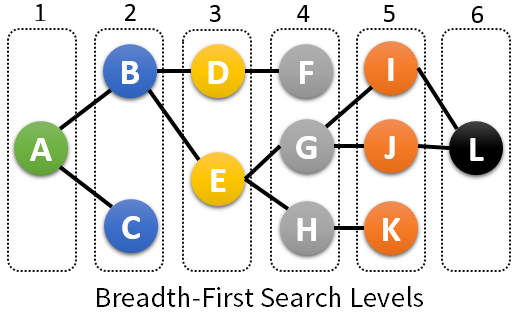
\includegraphics[width=8cm]{Term_2/Source/images/bfs_2_lvl.png}
    
Сложность по времени и памяти - ?

\end{frame}

\begin{frame}[fragile]{Взвешенный граф}
Что такое взвешенный граф?
    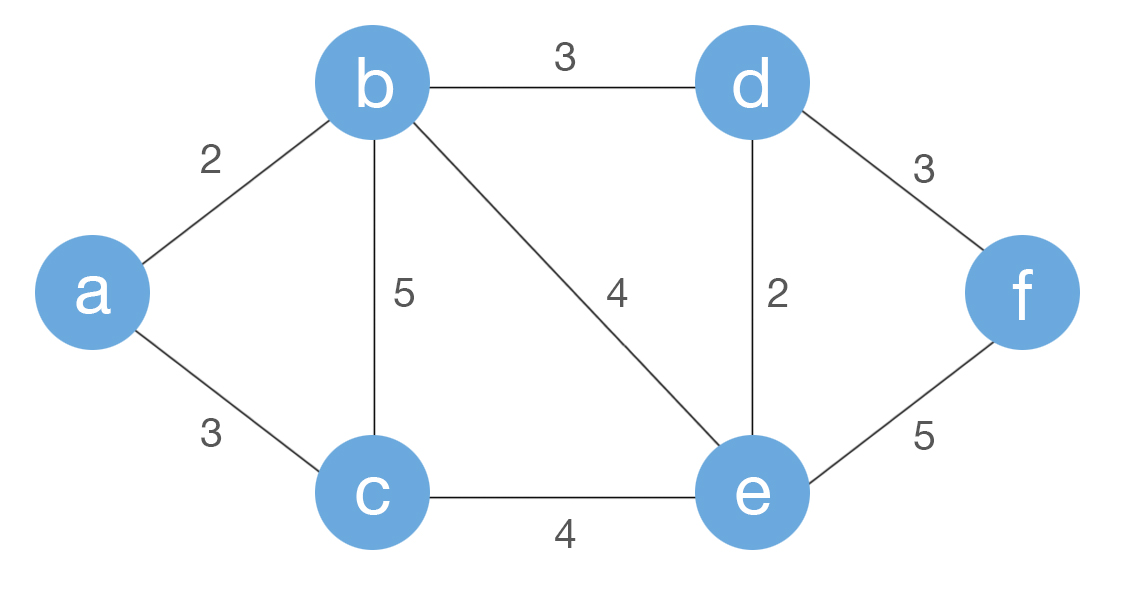
\includegraphics[width=8cm]{Term_2/Source/images/weigted_graph.jpg}
\end{frame}

\subsection{Граф 0-1. Кратчайшие пути}

\begin{frame}[fragile]{Взвешенный граф. Граф 0-1}
Частный случай взвешенного графа. Ребра имеют веса 0 и 1.

Кратчайший путь может быть найден модификацией BFS.
    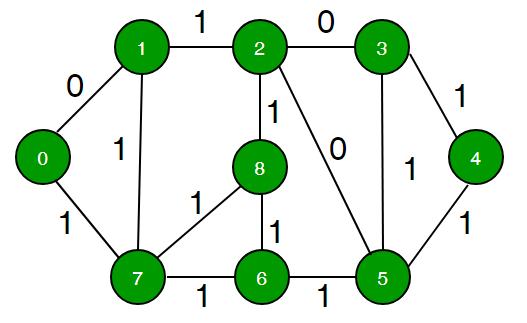
\includegraphics[width=8cm]{Term_2/Source/images/binary-graph.png}
    
\end{frame}

\begin{frame}[fragile]{Взвешенный граф. Граф 0-1}
Нам поможет структура данных deque.
    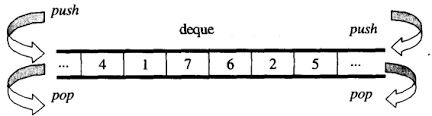
\includegraphics[width=8cm]{Term_2/Source/images/deque.png}
    
Напоминание.

Стандартная библиотека: std::deque.
    \begin{itemize}
        \item push\_back - добавление в конец
        \item pop\_back - получение из конца
        \item push\_front - добавление в начало
        \item pop\_front - получение из начала
    \end{itemize}

\end{frame}

\begin{frame}[fragile]{Взвешенный граф. Граф 0-1}
Если найдена необработанная вершина, то делаем проверку, чему равен вес ребра, который ведет к ней. Если 0 - добавление в начало очереди, 1 - в конец.

\begin{lstlisting}

    if (dist[edges[v][i].to] > dist[v] + edges[v][i].weight) 
    { 
        dist[edges[v][i].to] = dist[v] + edges[v][i].weight; 
    
        
        if (edges[v][i].weight == 0) 
            Q.push_front(edges[v][i].to); 
        else
            Q.push_back(edges[v][i].to); 
    }
\end{lstlisting}
\end{frame}
            
\subsection{Граф 1-K. Кратчайшие пути}

\begin{frame}[fragile]{Взвешенный граф. Граф 1-K}
Частный случай взвешенного графа. 
Веса всех ребер находятся в диапазоне 1-K.

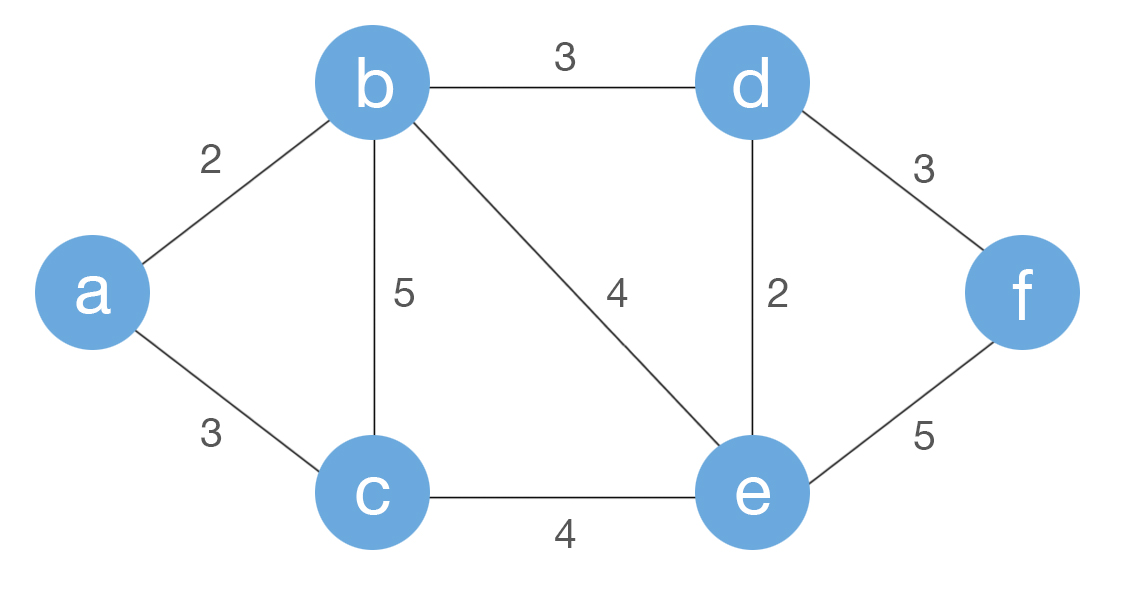
\includegraphics[width=8cm]{Term_2/Source/images/weigted_graph.jpg}
\end{frame}

\begin{frame}[fragile]{Взвешенный граф. Граф 1-K}
Наивное решение. 

Применим трансформацию графа: каждое ребро веса w>1 превратим в w ребер веса 1. Так мы превратили граф в обычный невзвешенный граф.

После этого запустим обычный BFS для поиска кратчайшего пути.

Временная сложность - O(E*k)

Память - O (E*k).

\end{frame}

\begin{frame}[fragile]{Взвешенный граф. Граф 1-K}
Альтернативное решение: k + 1 очередей\\
Временная сложность - O(E + V*k)\\
Память - O (V*k).

\end{frame}


\subsection{Алгоритм Дейкстры для поиска кратчайших путей}

\begin{frame}[fragile]{Алгоритм Дейкстры для поиска кратчайших путей}

\textbf{Важно}: допустимы только ребра неотрицательного веса 
    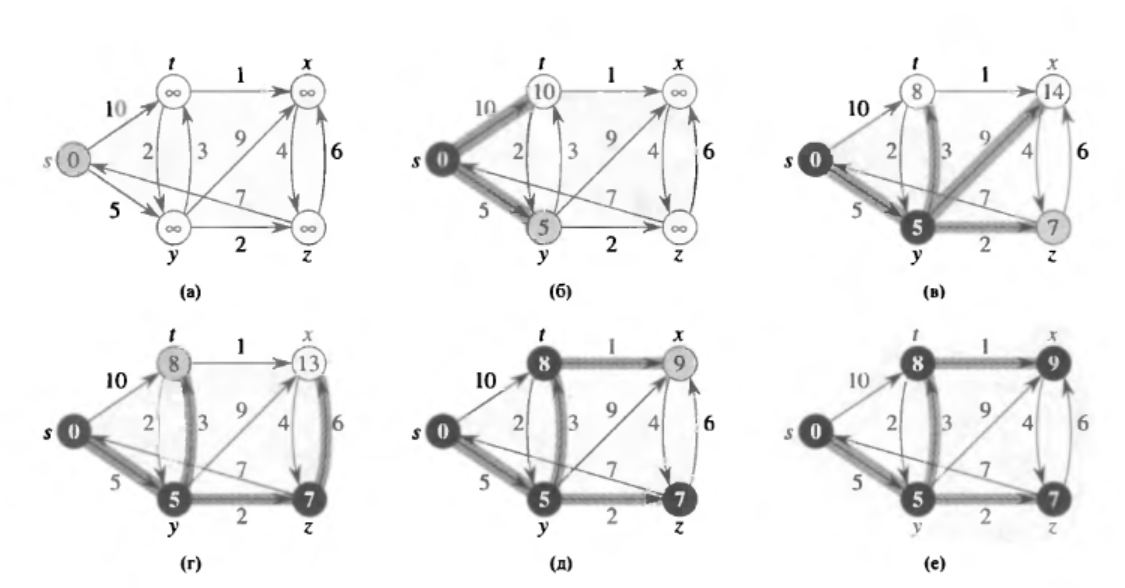
\includegraphics[width=12cm]{Term_2/Source/images/dijkstra.png}
\end{frame}


\subsection{Алгоритм Беллмана-Форда}

\begin{frame}[fragile]{Алгоритм Беллмана-Форда}
4 итераций обхода по числу вершин - 1
    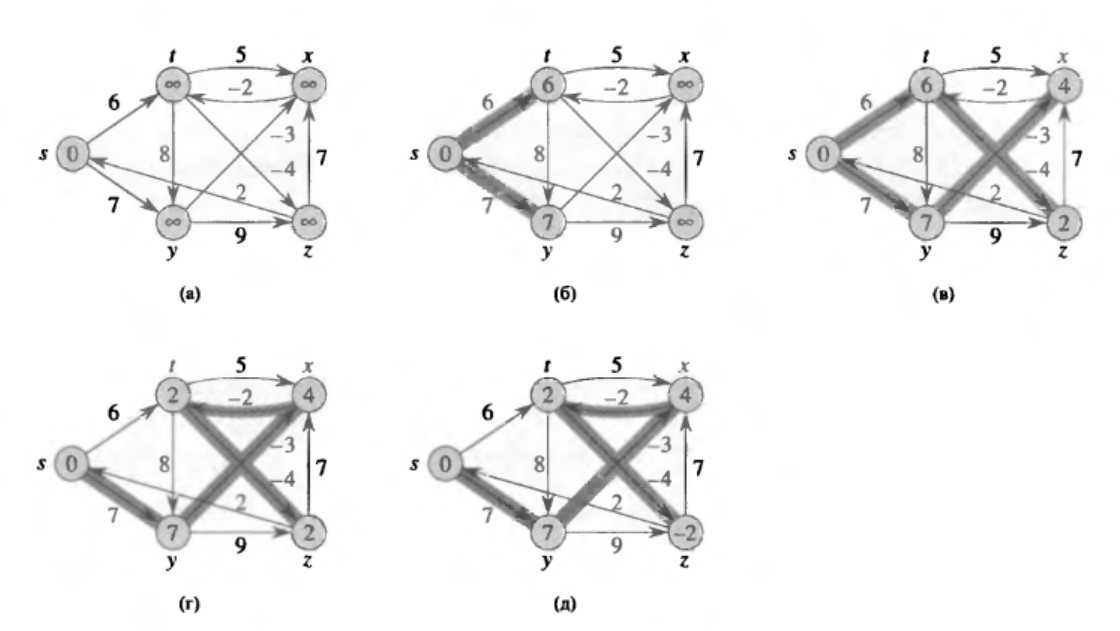
\includegraphics[width=12cm]{Term_2/Source/images/bellman-ford.png}

\end{frame}

\begin{frame}[fragile]{Алгоритм Беллмана-Форда: оптимизации}
\begin{enumerate}
    \item Остановка, если нет изменений в рёбрах
    \item Список обновлённых вершин
\end{enumerate}
\end{frame}

\appendix

\section<presentation>*{\appendixname}
\subsection<presentation>*{Useful links}

\end{document}


